
\chapter{Object Recognition by Stochastic Metric Learning}
\label{chap:metric} 



Descriptors extracted from deep neural networks have been shown to be very discriminative,
for example networks such as those trained on the large, very general ImageNet dataset have been used to extract descriptors robust for a variety of image classification tasks. Such retrieval systems utilise feature locality, for example Approximate Nearest Neighbour. Our goal is to use such descriptors as part of a large scale object instance recognition and retrieval system. We propose using deep nonlinear metric learning on Convolutional Neural Networks to learn features with good locality. In particular we worked with two related methods, \gls{NCA} and the related \gls{MEGM}.

We utilise a nonlinear form of \gls{MEGM} as an alternative to \gls{NCA} and propose some stochastic sampling methods to apply these (normally batch) methods to larger datasets with minibatch \gls{SGD}. On a larger scale we found the methods difficult to train, failing to converge or generalising very badly depending on training method or parameters. This led us to go back to a smaller dataset and examine the factors which lead to good generalization with this form of training.
  
We found on a small subset of the RGB-D dataset, surprisingly stochastic sampling methods generalised much better with small batch sizes, which acted as a form of regularisation. When trained with larger batches, or as a full batch, the dataset was over--fit. Given the correct parameters, descriptors extracted performed well at the Nearest Neighbour task and exceeded the performance of those extracted by applying standard supervised training.





\section{Introduction}

Deep convolutional neural networks in combination with modern \gls{GPU}s and large image datasets have shown strong performance on image classification tasks \cite {Krizhevsky2012}, and has been applied to related problems such as object detection \cite{Sermanet2013}, image segmentation \cite{Masci2013} and image retrieval \cite{Razavian2014}.

\subsection {Descriptors from Deep Neural Networks}

Using descriptors derived from the hidden layers of a neural networks trained using supervised learning, for the purpose of other learning tasks is a relatively new idea. These descriptors have been shown to be robust even for quite unrelated tasks \cite{Donahue2014,Razavian2014}. The ImageNet dataset \cite{Krizhevsky2012} is a popular source for pretraining, and pre-trained models exist such as the OverFeat network \cite{Sermanet2013} or the DeCAF feature extractor \cite{Donahue2014}). 

A standard technique in training a \gls{CNN} is to augment the dataset by applying transformations, more data typically gives better generalization. In \cite{Dosovitskiy2013}, a \gls{CNN} was trained on single images which were warped in many different ways. Features obtained from the network were then used in popular classification benchmarks achieving good results. For many years local image descriptors such as \gls{SIFT} \cite{Lowe2004} have been used for matching and indexing images, a recent comparison \cite{Fischer2014} (though perhaps not a fair one) showed that using a \gls{CNN} for matching tasks performed better than \gls{SIFT} by a margin similar to the improvement given by \gls{SIFT} to raw pixel data.


The final layer of a standard deep neural network as used in supervised classification consists of a set of linear classifiers, as such those descriptors are suitable for classification using other linear classifiers such as \gls{SVM}s. Nearest Neighbor suffers from high dimensionality and noisy or irrelevant dimensions, as such the descriptors produced by a CNN may not be suitable for comparison by distance. For that reason we have looked towards metric learning to directly optimise the descriptors for the purpose of Nearest Neighbor classification. 


\subsection {Deep Metric Learning}


Metric learning has often been used for object recognition and image classification \cite{Hadsell2006,Min2009} (and many others), and especially face recognition, for example \cite{Kostinger2012}. Although most efforts often have focused on mahalanobis distance metric learning (a form of distance metric learning linear transformation), deep metric learning has had some attention \cite {Salakhutdinov2007a,Min2009,Weston2009,Min2010}. At the expense of much larger computation cost, deep metric learning has been shown to perform much better than its linear counterparts. We use gradients from metric learning to drive \gls{SGD} on a deep \gls{CNN}. 

Siamese networks utilise shared parameters between two networks, and are used to perform comparisons between two examples at a time, usually for the purpose of descriptor learning. Our method generalises this to multiple examples at a time.

\subsection {Training}

Metric learning comes with its own set of challenges, it has often been formulated as batch training method because each example potentially interacts with every other example. In practice descriptors from examples far apart don't interact with each other at all, so approximations can be made as we discuss later. This runs into issues relating to high dimensional spaces, namely the ``curse of dimensionality''. In high dimensional spaces, such as those we deal with in this paper, if the points (descriptors) were uniformly spaced then on average the number of neighbours increases with dimension. 

The interaction between points decays with distance (for example exponentially with \gls{NCA}). We can use approximations around the local neighbourhood of examples which can be used to create an \gls{SGD} training procedure. Using an approximation to the nearest $ k $ neighbours is a popular approach, seen in \cite{Mensink2012,Zaidi2011} (of many). Clustering (amongst other sampling methods) is discussed in  \cite{Oneat2011} such as Farthest Point or Random Projection clustering, the downside of such clustering is that it is hard to control the size of a batch. 

Many training methods focus on interaction between pairs of (similar/dissimilar) examples or triples (example, more similar, less similar), for example DrLIM \cite{Hadsell2006} where a spring analogy is used to create an attraction between similar pairs and a repulsion between dissimilar pairs, the advantage with this kind method is that it can be used without explicit class labels, but just a similar/dissimilar annotation.

\section {Deep Metric Learning}

A deep neural network (in our case a \gls{CNN}) is used to to create an embedding into a lower dimensional space, creating descriptors which can be compared with their euclidean distance (and classified with nearest neighbour) where the euclidean distance of the raw pixels is both expensive and not a good measure of the distance of the semantic similarity of image content. 

We examine non linear versions of two methods \gls{NCA} \cite{Goldberger2004}, the closely related, but less well known \gls{MEGM} \cite {Zaidi2011}. \gls{NCA} optimizes a continuous version of the \gls{LOO} performance, it uses a softmax over weights which decay exponentially with distance. The \gls{NCA} score can be interpreted as the probability that a descriptor will pick another descriptor of the correct class as its nearest neighbour. 

The probability, $ p_{ij} $, of one descriptor selecting another descriptor, as its neighbour is defined as a softmax function over weights $W_ij$. The indexes $ i $ and $ j $ refer to input examples $x_i$ and $x_j$, and corresponding vector valued output of a \gls{CNN} $f(x_i)$ and $f(x_j)$ which are the descriptor vectors.

\begin{equation}
\label{eq:nca_prob_pair}
p_{ij} =  \frac {W_{ij}} {\sum_{k \neq i}{W_{ik}}}g
\end{equation}

Then the total probability, $ p_i $, of a point selecting any neighbour with another with its \emph{correct} class is defined as the sum of those neighbour probabilities $p_{ij}$ which have the same class:

\begin{equation}
\label{eq:nca_prob}
p_{i} =  \sum_{j:c_j = c_i}{p_{ij}}
\end{equation}

Where $ C_i $ is the class label of example $ i $. We use a gaussian kernel for the weighting as \cite{Zaidi2011} do. 

\begin{equation}
 \label{eq:gaussian_kernel}
W_{ij} = exp(\frac{-\lVert f(x_i) - f(x_j) \rVert^2_2 }{2\sigma^2}), \space W_{ii} = 0
\end{equation}


Then the function to be maximized, is the total sum of the probabilities of all descriptors being correctly classified.

\begin{equation}
\label{eq:nca_loss}
\mathcal{E}_{nca} =  \sum_i {p_i}
\end{equation}

Where \gls{NCA} optimises directly on the probability $ p_{i} $ above, \gls{MEGM} instead computes for each class $ \hat{y_{ti}} $ as a prediction that a descriptor will take class $ t $, where the only difference is that $ c_j = t $ as opposed to $ c_j = c_i $:

\begin{equation}
\label{eq:megm_pred}
\hat{y_{ti}} = \frac{\sum_{j:c_j = t}W_{ij}}{\sum_{k \neq i}{W_{ik}}}
\end{equation}

The prediction $ \hat{y_{ti}} $ can then be compared with $ y_{ti} $ (1 where $ t = c_i $, 0 otherwise), it then minimizes the \gls{MSE} between prediction and true class label:

\begin{equation}
\label{eq:megm_loss}
\mathcal{E}_{megm} =  \sum_i\sum_t{(y_{ti} - \hat{y_{ti}})^2}
\end{equation}

Intuitively \gls{MEGM} can be seen to penalize the case where two classes compete for the same region more so than when one class competes against examples of many different classes, where as \gls{NCA} would treat the two cases approximately equally. These loss functions can be used to drive gradient descent on a \gls{CNN} by standard backpropogation. The derivative for \gls{MEGM} is shown in the appendix, section~\ref{sec:appendix}.

We compute the gradient over the outputs of each minibatch and apply backpropogation as usual to find the derivative with respect to the weights of the network. It can be noted that the output, and derivative for \gls{MEGM} is more expensive to compute because of the additional per class summation, so it would not be suitable with an extremely large number of classes. In practice a large number of the terms can be factored out and precomputed, as well as computing the difference summations in terms of matrix multiplication.

Note the parameter $ \sigma $ was not in the original NCA, and is initialized to the average distance to the nearest neighbours of the initial descriptor output before training. We use it to prevent the weights initializing to zero when the distance between descriptors is large.


Where $\alpha $ controls the trade-off. When $ \alpha \mathcal{E}_{mse} > \mathcal{E}_{nca} $ the descriptors all collapse into the same point.


\section{SGD for metric learning}

Our main proposal is in using minibatch \gls{SGD}, and applying it to metric learning methods which have been designed as batch learning methods. Metric learning as shown above as a batch method, scales at $ O(n^2) $ for $ n $ examples. Given that we wish to apply these approaches to large datasets containing hundreds of thousands or millions of images we are forced to consider approximations. The typical method for training a \gls{CNN} on large numbers of images is using \gls{SGD}, because it is fast, simple and scales to handle large datasets easily. 

The most obvious approximation is to just truncate the influence to the nearest $ k $ neighbours as the weight exponentially decays with the square distance. We hypothesised this would lead to the best approximation, however there are many ways of truncating the neighbourhoods. This lends itself to clustering methods and is more complicated than the alternative, which is to sample batches randomly, but use a large enough batch to include several examples of each class.

We propose the following approaches for sampling batches for \gls{SGD}:

\begin{enumerate}
\item {\bf Random shuffled batches}
 Randomly shuffle the dataset and divide up into batches of a fixed size, exactly how batches would normally be selected for supervised learning. Each batch contains (almost certainly) different numbers of examples from each class.
 \item {\bf Stratified random batches} 
 Pick batches by selecting a number of examples from each class, to ensure the same number of examples of each class are represented in each batch.   

 \item {\bf K-neighbourhoods around random points}
 Before each training epoch, run the model forward through the training set to obtain descriptors for each example. Select N examples at random and pick the batch as the batch sized neighbourhood (in descriptor space) of each selected example.
\end {enumerate}


\subsection {Issues of Scale}

The parameter $ \sigma $ is largely optional in theory, as the scale can be factored into the final fully connected weight matrix (or previous layers).  We make use of $ \sigma $ for the purposes of numerical stability upon initialization, during training the density of points adjusts itself to fit this parameter. It can also be observed that for different values of $ \sigma $ that the distance between descriptors adjust themselves to fit the new parameter over a few iterations of training.


\subsection {Adding Mean Square Error}

We experimented with adding the square distance between members of the same class as a means of adding some bias to the loss functions after suspecting that metric learning methods decribed above were overfitting, to force the output distribution to be more simple. 

\begin{equation}
\label{eqn:mse}
\mathcal{E}_{mse} = \sum_i{ \sum_{j:j_c = i_c}  \frac {{\lVert f(x_i) - f(x_j) \rVert^2_2}} {\sigma^2} }
\end{equation}

\begin{equation}
\label{eqn:mse_total}
\mathcal{E}_{total} =  \mathcal{E}_{nca} + \alpha \mathcal{E}_{mse}
\end{equation}


\subsection {kNN implementation}

We use a brute force \gls{KNN} algorithm running on CUDA \cite{Garcia2008}, computing the distance matrix using matrix multiplication followed by using an insertion sort to select the $ k $ neighbours of lowest distance. This approach is not scaleable to large datasets, and smarter clustering algorithms will eventually need to be used, however the time for evaluating \gls{KNN} on the datasets we experimented with are still dominated by the cost of computing descriptors from examples. 


\section {CNN architecture}


\begin{figure}[ht]
\centering
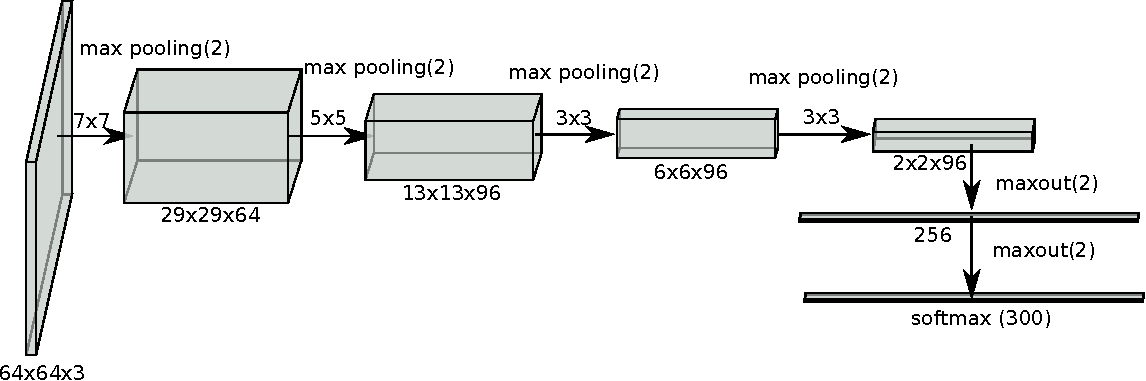
\includegraphics[width=1\textwidth]{metric_learning/convnet.pdf}
\caption{Convolutional network configuration used for $64\times64$ rgb images with supervised learning.}
\label{fig:metric_convnet}
\end{figure}

We used a fairly standard convolutional neural network of six layers, with four layers of convolution and max pooling using rectified linear activation functions, two fully connected layers using maxout \cite{Springenberg2013} units as an activation method, shown in Figure~\ref{fig:metric_convnet}. Dropout \cite{HintonDropout} with a rate of $ 0.5 $ is used when training on inputs to the two fully connected layers. For metric learning, the last linear layer and softmax are removed, leaving four convolutional layers and a single fully connected layer giving descriptors of size $ 256 $.

Dropout and Maxout have been shown to be beneficial in a supervised learning scenario for the purposes regularization. In the standard supervised training scenario Dropout is of great practical use because it (to some degree) prevents overfitting, and mostly does away with the need for early stopping. However we found that it prevented good generalization when used with metric learning approaches.

\subsection {Data augmentation}

\begin{figure}[h]
\centering
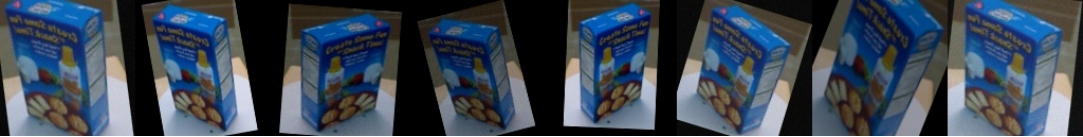
\includegraphics[width=1\textwidth]{metric_learning/augmentation.png}
\caption{Example of image distortions resulting from transformations of a single source image}
\label{fig:metric_augmentation}
\end{figure}


In all cases we used randomized data augmentation of the test set by applying random distortions to ensure the network never saw exactly the same image twice, and to increase its tolerance to small changes in lighting, translation and rotation. The parameters of the data augmenmtation can be seen in Figure \ref{fig:metric_permute}. Without the data augmenmtation supervised training produces substantially worse generalization than without in both supervised and metric learning approaches. In all experiments testing was performed on non-distorted images and trained with distorted images.

\begin{table*}
  \centering
    \caption{Ranges of parameters used for image distortion }

  \begin{tabular}{ l  l }
    \toprule
    scale (uniform) & $ 1 \pm 0.2 $  \\ 
    squash  & $ 1 \pm 0.2 $  \\ 
    rotation (rads) & $ \pm \frac{\pi}{16} $ \\ 
    translation(x, y) (\% image size) & $ \pm 5 \% $ \\ 
    brightness (additive) & $ \pm 20 \% $ \\ 
    contrast (multiplicative) & $ 1 \pm 0.2 \% $ \\ 
    gaussian pixel noise & $ \sigma = 2 \pm 2 $  \\ 
    flip horizontal (probability) & $ 0.5 $ \\ 
    \bottomrule
  \end{tabular}
\label{fig:metric_permute}
\end{table*}

\subsection {Dataset}

\begin{figure}[h]
\centering
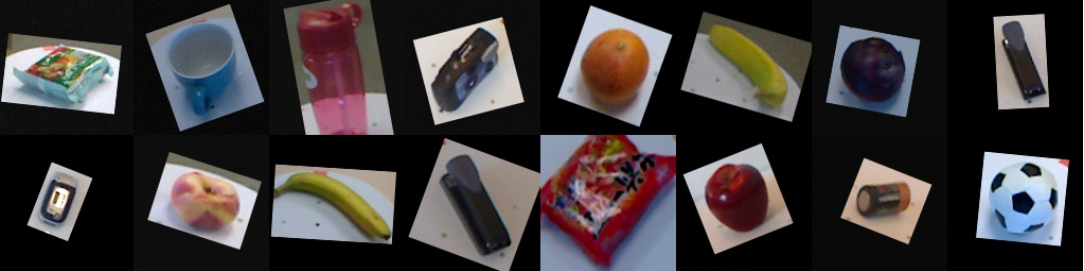
\includegraphics[width=1\textwidth]{metric_learning/objects.png}
\caption{Samples of images used in training from different objects}
\label{fig:metric_dataset}
\end{figure}

We experimented with the University of Washington RGB-D dataset primarily because it has a standard test set for instance recognition and a large number of published results, it contains 300 objects from 50 classes. Each object has 3 sequences of rotations at 30, 45 and 60 degrees elevation, each rotation sequence contains approximately 150 images. For instance recognition the sequence at 30 and 60 degrees are used for training and the sequence at 45 degrees is used for testing. 

We used a cut down version of the RGB-D dataset for a number of experiments, with 50 objects and 100 images of each object to train on, and 50 images per object to test. The images were randomly selected.

We used a resolution of $ 64\times64 $ on the RGB-D images, we used the cropped version of the data, our procedure for re-sizing was to load all of the images in a sequence and if any image was at a higher resolution than $ 72\times72 $ we re-sized the image to $ 72\times72 $ and all other images in the sequence by the same ratio. The images were then distorted (see Figure~\ref{fig:metric_permute}) and finally centred (modulo translation) on a  $ 64\times64 $ with a black background.


\section {Experiments}


In all cases (unless otherwise specified) we use a minibatch size of 256, with standard \gls{SGD} learning rate set to $ 10^{-2} $ for supervised learning, and $ 10^{-5} $ for metric learning methods. We experimented with other learning rates for metric learning, in some cases a lower learning rate of $ 10^{-6} $ was used when the higher rate caused divergence.

We manually divided the training rate by a factor of 10 when the training set accuracy plateaus for supervised learning. Supervised learning methods greatly benefit from reducing the learning rate after time, however we did not notice any benefit to the metric learning methods. Metric learning methods we stopped at 70 epochs, or earlier if they were not converging. Overall we found \gls{MEGM} to give similar, but slightly better test set accuracy than \gls{NCA}, we performed most experiments with \gls{MEGM} for consistency.



\subsection{Overall Comparison}

We compare the testing classification error between methods, the final accuracy
is reported as the test set classification accuracy average over the last 5 iterations.
Test set accuracy is percentage accuracy for supervised learning, and for metric
learning by $k = 5$ nearest neighbours and selecting the most common class.




\begin{table*}[ht]

\centering
  \caption{Summary of training methods}

  \begin{tabular}{  l l  l  l l l }
  
    \toprule
    Method &  Sampling & Batch  & Test accuracy &  Train epochs \\  \hline
    \bf{Initialisation} & &  &  $ 64.0  $ & 0  &  \\  
    \hline
    
    \bf{Supervised} & & 256 &  $ 90.6  $ & 40  &  \\  
     & 5NN  &  &  $ 89.0  $ & 40 &  \\  
     \hline
    
    \bf{NCA} &  & batch &  $  71.2  $ &  50  & \\
     & random & 256 & $  94.0  $ & 70 & \\
    
    \hline
    
    \bf{MEGM} &  & batch  &  $  74.4  $ &  50  & \\
     & random & 128 &  $  95.0  $ &  70  & \\     
     &  & 256 & $  90.5  $ &  70 & \\  
     &  & 512 & $  81.4  $ &  70 & \\
    
    \hline
    \bf{MEGM} & stratified & 128 & $  {\bf 95.4 }  $ & 70 & \\  
    
     &  & 256 & $  94.6  $ & 70 & \\  
     &  & 512 & $  87.1  $ & 70 & \\  

     \hline
     
    \bf{MEGM} & neighbourhoods & 256 & $  80.4  $ & 70  & \\
    
    \hline
    
    \bf{MEGM + MSE} & stratified & 128 & $  {\bf 95.3 }  $ & 70  & \\

      \bottomrule
    
    \end{tabular}
\label{fig:metric_summary}
\end{table*}



We sought to compare the sampling approximation to the batch method.
As a batch method, clearly \gls{SGD} is not the ideal training method. We were
surprised to see that despite the loss function smoothly decreasing (as can be
seen in Figure~\ref{fig:metric_megm_test}), training failed to generalise well to the training set Figure~\ref{fig:metric_megm_loss}.
We anticipated the batch metric learning methods would work best as batch
methods or with larger batches (as closer approximations to the batch method).
We can see that is not the case, and both the batch method and \gls{SGD} with the
larger batch size (512) both failed to generalise well. The same pattern occurred
for \gls{NCA}, as well as using the stratified sampling method.
The reason for such over-fitting is that we believe the two metric learning
methods to have not enough bias to force the network to learn something. \gls{NCA}
allows highly complex and multimodal distributions with many local minima
which, provided the local neighbourhood structure fits, are not penalised by it’s
loss function. Smaller batch sizes however act as a regularisation, forcing the
descriptors outputs to a simpler form.



\begin{figure}[ht]
   \begin{tikzpicture}[gnuplot]
%% generated with GNUPLOT 4.6p1 (Lua 5.1; terminal rev. 99, script rev. 100)
%% Thu 31 Jul 2014 02:53:39 NZST
\gpsolidlines
\path (0.000,0.000) rectangle (12.700,7.620);
\gpcolor{color=gp lt color axes}
\gpsetlinetype{gp lt axes}
\gpsetlinewidth{1.00}
\draw[gp path] (1.504,0.985)--(12.147,0.985);
\gpcolor{color=gp lt color border}
\gpsetlinetype{gp lt border}
\draw[gp path] (1.504,0.985)--(1.684,0.985);
\draw[gp path] (12.147,0.985)--(11.967,0.985);
\node[gp node right] at (1.320,0.985) { 0};
\gpcolor{color=gp lt color axes}
\gpsetlinetype{gp lt axes}
\draw[gp path] (1.504,1.556)--(12.147,1.556);
\gpcolor{color=gp lt color border}
\gpsetlinetype{gp lt border}
\draw[gp path] (1.504,1.556)--(1.684,1.556);
\draw[gp path] (12.147,1.556)--(11.967,1.556);
\node[gp node right] at (1.320,1.556) { 0.1};
\gpcolor{color=gp lt color axes}
\gpsetlinetype{gp lt axes}
\draw[gp path] (1.504,2.127)--(12.147,2.127);
\gpcolor{color=gp lt color border}
\gpsetlinetype{gp lt border}
\draw[gp path] (1.504,2.127)--(1.684,2.127);
\draw[gp path] (12.147,2.127)--(11.967,2.127);
\node[gp node right] at (1.320,2.127) { 0.2};
\gpcolor{color=gp lt color axes}
\gpsetlinetype{gp lt axes}
\draw[gp path] (1.504,2.698)--(12.147,2.698);
\gpcolor{color=gp lt color border}
\gpsetlinetype{gp lt border}
\draw[gp path] (1.504,2.698)--(1.684,2.698);
\draw[gp path] (12.147,2.698)--(11.967,2.698);
\node[gp node right] at (1.320,2.698) { 0.3};
\gpcolor{color=gp lt color axes}
\gpsetlinetype{gp lt axes}
\draw[gp path] (1.504,3.269)--(12.147,3.269);
\gpcolor{color=gp lt color border}
\gpsetlinetype{gp lt border}
\draw[gp path] (1.504,3.269)--(1.684,3.269);
\draw[gp path] (12.147,3.269)--(11.967,3.269);
\node[gp node right] at (1.320,3.269) { 0.4};
\gpcolor{color=gp lt color axes}
\gpsetlinetype{gp lt axes}
\draw[gp path] (1.504,3.840)--(12.147,3.840);
\gpcolor{color=gp lt color border}
\gpsetlinetype{gp lt border}
\draw[gp path] (1.504,3.840)--(1.684,3.840);
\draw[gp path] (12.147,3.840)--(11.967,3.840);
\node[gp node right] at (1.320,3.840) { 0.5};
\gpcolor{color=gp lt color axes}
\gpsetlinetype{gp lt axes}
\draw[gp path] (1.504,4.411)--(12.147,4.411);
\gpcolor{color=gp lt color border}
\gpsetlinetype{gp lt border}
\draw[gp path] (1.504,4.411)--(1.684,4.411);
\draw[gp path] (12.147,4.411)--(11.967,4.411);
\node[gp node right] at (1.320,4.411) { 0.6};
\gpcolor{color=gp lt color axes}
\gpsetlinetype{gp lt axes}
\draw[gp path] (1.504,4.982)--(12.147,4.982);
\gpcolor{color=gp lt color border}
\gpsetlinetype{gp lt border}
\draw[gp path] (1.504,4.982)--(1.684,4.982);
\draw[gp path] (12.147,4.982)--(11.967,4.982);
\node[gp node right] at (1.320,4.982) { 0.7};
\gpcolor{color=gp lt color axes}
\gpsetlinetype{gp lt axes}
\draw[gp path] (1.504,5.553)--(9.759,5.553);
\draw[gp path] (11.963,5.553)--(12.147,5.553);
\gpcolor{color=gp lt color border}
\gpsetlinetype{gp lt border}
\draw[gp path] (1.504,5.553)--(1.684,5.553);
\draw[gp path] (12.147,5.553)--(11.967,5.553);
\node[gp node right] at (1.320,5.553) { 0.8};
\gpcolor{color=gp lt color axes}
\gpsetlinetype{gp lt axes}
\draw[gp path] (1.504,6.124)--(9.759,6.124);
\draw[gp path] (11.963,6.124)--(12.147,6.124);
\gpcolor{color=gp lt color border}
\gpsetlinetype{gp lt border}
\draw[gp path] (1.504,6.124)--(1.684,6.124);
\draw[gp path] (12.147,6.124)--(11.967,6.124);
\node[gp node right] at (1.320,6.124) { 0.9};
\gpcolor{color=gp lt color axes}
\gpsetlinetype{gp lt axes}
\draw[gp path] (1.504,6.695)--(12.147,6.695);
\gpcolor{color=gp lt color border}
\gpsetlinetype{gp lt border}
\draw[gp path] (1.504,6.695)--(1.684,6.695);
\draw[gp path] (12.147,6.695)--(11.967,6.695);
\node[gp node right] at (1.320,6.695) { 1};
\gpcolor{color=gp lt color axes}
\gpsetlinetype{gp lt axes}
\draw[gp path] (1.504,0.985)--(1.504,6.695);
\gpcolor{color=gp lt color border}
\gpsetlinetype{gp lt border}
\draw[gp path] (1.504,0.985)--(1.504,1.165);
\draw[gp path] (1.504,6.695)--(1.504,6.515);
\node[gp node center] at (1.504,0.677) { 0};
\gpcolor{color=gp lt color axes}
\gpsetlinetype{gp lt axes}
\draw[gp path] (3.024,0.985)--(3.024,6.695);
\gpcolor{color=gp lt color border}
\gpsetlinetype{gp lt border}
\draw[gp path] (3.024,0.985)--(3.024,1.165);
\draw[gp path] (3.024,6.695)--(3.024,6.515);
\node[gp node center] at (3.024,0.677) { 10};
\gpcolor{color=gp lt color axes}
\gpsetlinetype{gp lt axes}
\draw[gp path] (4.545,0.985)--(4.545,6.695);
\gpcolor{color=gp lt color border}
\gpsetlinetype{gp lt border}
\draw[gp path] (4.545,0.985)--(4.545,1.165);
\draw[gp path] (4.545,6.695)--(4.545,6.515);
\node[gp node center] at (4.545,0.677) { 20};
\gpcolor{color=gp lt color axes}
\gpsetlinetype{gp lt axes}
\draw[gp path] (6.065,0.985)--(6.065,6.695);
\gpcolor{color=gp lt color border}
\gpsetlinetype{gp lt border}
\draw[gp path] (6.065,0.985)--(6.065,1.165);
\draw[gp path] (6.065,6.695)--(6.065,6.515);
\node[gp node center] at (6.065,0.677) { 30};
\gpcolor{color=gp lt color axes}
\gpsetlinetype{gp lt axes}
\draw[gp path] (7.586,0.985)--(7.586,6.695);
\gpcolor{color=gp lt color border}
\gpsetlinetype{gp lt border}
\draw[gp path] (7.586,0.985)--(7.586,1.165);
\draw[gp path] (7.586,6.695)--(7.586,6.515);
\node[gp node center] at (7.586,0.677) { 40};
\gpcolor{color=gp lt color axes}
\gpsetlinetype{gp lt axes}
\draw[gp path] (9.106,0.985)--(9.106,6.695);
\gpcolor{color=gp lt color border}
\gpsetlinetype{gp lt border}
\draw[gp path] (9.106,0.985)--(9.106,1.165);
\draw[gp path] (9.106,6.695)--(9.106,6.515);
\node[gp node center] at (9.106,0.677) { 50};
\gpcolor{color=gp lt color axes}
\gpsetlinetype{gp lt axes}
\draw[gp path] (10.627,0.985)--(10.627,5.283);
\draw[gp path] (10.627,6.515)--(10.627,6.695);
\gpcolor{color=gp lt color border}
\gpsetlinetype{gp lt border}
\draw[gp path] (10.627,0.985)--(10.627,1.165);
\draw[gp path] (10.627,6.695)--(10.627,6.515);
\node[gp node center] at (10.627,0.677) { 60};
\gpcolor{color=gp lt color axes}
\gpsetlinetype{gp lt axes}
\draw[gp path] (12.147,0.985)--(12.147,6.695);
\gpcolor{color=gp lt color border}
\gpsetlinetype{gp lt border}
\draw[gp path] (12.147,0.985)--(12.147,1.165);
\draw[gp path] (12.147,6.695)--(12.147,6.515);
\node[gp node center] at (12.147,0.677) { 70};
\draw[gp path] (1.504,6.695)--(1.504,0.985)--(12.147,0.985)--(12.147,6.695)--cycle;
\node[gp node center,rotate=-270] at (0.246,3.840) {Loss function};
\node[gp node center] at (6.825,0.215) {Epoch};
\node[gp node center] at (6.825,7.157) {Effect of batch size on training};
\node[gp node right] at (10.679,6.361) {batch};
\gpcolor{color=gp lt color 0}
\gpsetlinetype{gp lt plot 0}
\draw[gp path] (10.863,6.361)--(11.779,6.361);
\draw[gp path] (1.656,4.618)--(1.808,3.418)--(1.960,3.033)--(2.112,2.821)--(2.264,2.610)%
  --(2.416,2.426)--(2.568,2.286)--(2.720,2.213)--(2.872,2.117)--(3.024,1.984)--(3.176,1.944)%
  --(3.329,1.897)--(3.481,1.981)--(3.633,1.874)--(3.785,1.800)--(3.937,1.778)--(4.089,1.778)%
  --(4.241,1.829)--(4.393,1.621)--(4.545,1.620)--(4.697,1.603)--(4.849,1.583)--(5.001,1.610)%
  --(5.153,1.571)--(5.305,1.508)--(5.457,1.543)--(5.609,1.478)--(5.761,1.464)--(5.913,1.397)%
  --(6.065,1.392)--(6.217,1.415)--(6.369,1.428)--(6.521,1.377)--(6.673,1.339)--(6.826,1.336)%
  --(6.978,1.319)--(7.130,1.323)--(7.282,1.311)--(7.434,1.281)--(7.586,1.285)--(7.738,1.269)%
  --(7.890,1.236)--(8.042,1.239)--(8.194,1.246)--(8.346,1.220)--(8.498,1.237)--(8.650,1.234)%
  --(8.802,1.224)--(8.954,1.224)--(9.106,1.229)--(9.258,1.213)--(9.410,1.195)--(9.562,1.219)%
  --(9.714,1.183)--(9.866,1.182)--(10.018,1.178)--(10.170,1.178)--(10.322,1.180)--(10.475,1.156)%
  --(10.627,1.154)--(10.779,1.163)--(10.931,1.147)--(11.083,1.130)--(11.235,1.170)--(11.387,1.161)%
  --(11.539,1.148)--(11.691,1.148)--(11.843,1.136)--(11.995,1.138)--(12.147,1.178);
\gpcolor{color=gp lt color border}
\node[gp node right] at (10.679,6.053) {512};
\gpcolor{color=gp lt color 1}
\gpsetlinetype{gp lt plot 1}
\draw[gp path] (10.863,6.053)--(11.779,6.053);
\draw[gp path] (1.656,5.309)--(1.808,4.196)--(1.960,3.211)--(2.112,3.002)--(2.264,2.943)%
  --(2.416,2.572)--(2.568,2.593)--(2.720,2.390)--(2.872,2.548)--(3.024,2.452)--(3.176,2.414)%
  --(3.329,2.647)--(3.481,2.362)--(3.633,2.350)--(3.785,2.403)--(3.937,2.347)--(4.089,2.226)%
  --(4.241,2.214)--(4.393,1.957)--(4.545,1.999)--(4.697,1.932)--(4.849,1.826)--(5.001,1.860)%
  --(5.153,1.942)--(5.305,1.952)--(5.457,2.000)--(5.609,1.978)--(5.761,1.900)--(5.913,1.980)%
  --(6.065,2.118)--(6.217,2.145)--(6.369,1.926)--(6.521,1.853)--(6.673,1.912)--(6.826,1.888)%
  --(6.978,1.804)--(7.130,1.620)--(7.282,1.626)--(7.434,1.582)--(7.586,1.623)--(7.738,1.676)%
  --(7.890,1.607)--(8.042,1.690)--(8.194,1.609)--(8.346,1.633)--(8.498,1.652)--(8.650,1.496)%
  --(8.802,1.542)--(8.954,1.581)--(9.106,1.530);
\gpcolor{color=gp lt color border}
\node[gp node right] at (10.679,5.745) {256};
\gpcolor{color=gp lt color 2}
\gpsetlinetype{gp lt plot 2}
\draw[gp path] (10.863,5.745)--(11.779,5.745);
\draw[gp path] (1.656,4.467)--(1.808,3.418)--(1.960,3.034)--(2.112,2.795)--(2.264,2.683)%
  --(2.416,2.486)--(2.568,2.405)--(2.720,2.289)--(2.872,2.228)--(3.024,2.110)--(3.176,2.035)%
  --(3.329,1.990)--(3.481,1.969)--(3.633,2.010)--(3.785,1.904)--(3.937,1.844)--(4.089,1.816)%
  --(4.241,1.763)--(4.393,1.709)--(4.545,1.642)--(4.697,1.687)--(4.849,1.723)--(5.001,1.631)%
  --(5.153,1.654)--(5.305,1.597)--(5.457,1.640)--(5.609,1.651)--(5.761,1.586)--(5.913,1.517)%
  --(6.065,1.526)--(6.217,1.518)--(6.369,1.525)--(6.521,1.487)--(6.673,1.475)--(6.826,1.496)%
  --(6.978,1.450)--(7.130,1.421)--(7.282,1.401)--(7.434,1.448)--(7.586,1.408)--(7.738,1.382)%
  --(7.890,1.390)--(8.042,1.374)--(8.194,1.373)--(8.346,1.414)--(8.498,1.321)--(8.650,1.372)%
  --(8.802,1.323)--(8.954,1.331)--(9.106,1.332)--(9.258,1.289)--(9.410,1.283)--(9.562,1.297)%
  --(9.714,1.306)--(9.866,1.269)--(10.018,1.278)--(10.170,1.285)--(10.322,1.310)--(10.475,1.340)%
  --(10.627,1.321)--(10.779,1.287)--(10.931,1.257)--(11.083,1.269)--(11.235,1.279)--(11.387,1.272)%
  --(11.539,1.260)--(11.691,1.253)--(11.843,1.215)--(11.995,1.223)--(12.147,1.231);
\gpcolor{color=gp lt color border}
\node[gp node right] at (10.679,5.437) {128};
\gpcolor{color=gp lt color 3}
\gpsetlinetype{gp lt plot 3}
\draw[gp path] (10.863,5.437)--(11.779,5.437);
\draw[gp path] (1.656,6.572)--(1.808,6.442)--(1.960,6.047)--(2.112,5.805)--(2.264,4.617)%
  --(2.416,4.256)--(2.568,3.992)--(2.720,3.976)--(2.872,3.698)--(3.024,3.666)--(3.176,3.464)%
  --(3.329,3.415)--(3.481,3.399)--(3.633,3.232)--(3.785,3.263)--(3.937,3.247)--(4.089,3.028)%
  --(4.241,2.857)--(4.393,2.915)--(4.545,2.878)--(4.697,2.809)--(4.849,2.812)--(5.001,2.879)%
  --(5.153,2.762)--(5.305,2.641)--(5.457,2.670)--(5.609,2.569)--(5.761,2.666)--(5.913,2.492)%
  --(6.065,2.432)--(6.217,2.356)--(6.369,2.376)--(6.521,2.312)--(6.673,2.331)--(6.826,2.515)%
  --(6.978,2.388)--(7.130,2.271)--(7.282,2.293)--(7.434,2.301)--(7.586,2.211)--(7.738,2.336)%
  --(7.890,2.219)--(8.042,2.230)--(8.194,2.135)--(8.346,2.145)--(8.498,2.148)--(8.650,2.101)%
  --(8.802,2.042)--(8.954,2.068)--(9.106,2.128)--(9.258,2.040)--(9.410,2.013)--(9.562,1.977)%
  --(9.714,1.972)--(9.866,1.949)--(10.018,1.981)--(10.170,2.074)--(10.322,1.988)--(10.475,1.934)%
  --(10.627,1.890)--(10.779,1.864)--(10.931,1.879)--(11.083,1.847)--(11.235,1.878)--(11.387,1.821)%
  --(11.539,1.796)--(11.691,1.820)--(11.843,1.831)--(11.995,1.845)--(12.147,1.822);
\gpcolor{color=gp lt color border}
\gpsetlinetype{gp lt border}
\draw[gp path] (1.504,6.695)--(1.504,0.985)--(12.147,0.985)--(12.147,6.695)--cycle;
%% coordinates of the plot area
\gpdefrectangularnode{gp plot 1}{\pgfpoint{1.504cm}{0.985cm}}{\pgfpoint{12.147cm}{6.695cm}}
\end{tikzpicture}
%% gnuplot variables

   \caption{Loss function for different batch sizes, MEGM loss}
   \label {fig:metric_megm_loss}
\end{figure}

\begin{figure}[ht]
   \begin{tikzpicture}[gnuplot]
%% generated with GNUPLOT 4.6p1 (Lua 5.1; terminal rev. 99, script rev. 100)
%% Thu 31 Jul 2014 02:53:39 NZST
\gpsolidlines
\path (0.000,0.000) rectangle (12.700,7.620);
\gpcolor{color=gp lt color axes}
\gpsetlinetype{gp lt axes}
\gpsetlinewidth{1.00}
\draw[gp path] (1.320,0.985)--(12.147,0.985);
\gpcolor{color=gp lt color border}
\gpsetlinetype{gp lt border}
\draw[gp path] (1.320,0.985)--(1.500,0.985);
\draw[gp path] (12.147,0.985)--(11.967,0.985);
\node[gp node right] at (1.136,0.985) { 0};
\gpcolor{color=gp lt color axes}
\gpsetlinetype{gp lt axes}
\draw[gp path] (1.320,1.699)--(12.147,1.699);
\gpcolor{color=gp lt color border}
\gpsetlinetype{gp lt border}
\draw[gp path] (1.320,1.699)--(1.500,1.699);
\draw[gp path] (12.147,1.699)--(11.967,1.699);
\node[gp node right] at (1.136,1.699) { 5};
\gpcolor{color=gp lt color axes}
\gpsetlinetype{gp lt axes}
\draw[gp path] (1.320,2.413)--(12.147,2.413);
\gpcolor{color=gp lt color border}
\gpsetlinetype{gp lt border}
\draw[gp path] (1.320,2.413)--(1.500,2.413);
\draw[gp path] (12.147,2.413)--(11.967,2.413);
\node[gp node right] at (1.136,2.413) { 10};
\gpcolor{color=gp lt color axes}
\gpsetlinetype{gp lt axes}
\draw[gp path] (1.320,3.126)--(12.147,3.126);
\gpcolor{color=gp lt color border}
\gpsetlinetype{gp lt border}
\draw[gp path] (1.320,3.126)--(1.500,3.126);
\draw[gp path] (12.147,3.126)--(11.967,3.126);
\node[gp node right] at (1.136,3.126) { 15};
\gpcolor{color=gp lt color axes}
\gpsetlinetype{gp lt axes}
\draw[gp path] (1.320,3.840)--(12.147,3.840);
\gpcolor{color=gp lt color border}
\gpsetlinetype{gp lt border}
\draw[gp path] (1.320,3.840)--(1.500,3.840);
\draw[gp path] (12.147,3.840)--(11.967,3.840);
\node[gp node right] at (1.136,3.840) { 20};
\gpcolor{color=gp lt color axes}
\gpsetlinetype{gp lt axes}
\draw[gp path] (1.320,4.554)--(12.147,4.554);
\gpcolor{color=gp lt color border}
\gpsetlinetype{gp lt border}
\draw[gp path] (1.320,4.554)--(1.500,4.554);
\draw[gp path] (12.147,4.554)--(11.967,4.554);
\node[gp node right] at (1.136,4.554) { 25};
\gpcolor{color=gp lt color axes}
\gpsetlinetype{gp lt axes}
\draw[gp path] (1.320,5.268)--(12.147,5.268);
\gpcolor{color=gp lt color border}
\gpsetlinetype{gp lt border}
\draw[gp path] (1.320,5.268)--(1.500,5.268);
\draw[gp path] (12.147,5.268)--(11.967,5.268);
\node[gp node right] at (1.136,5.268) { 30};
\gpcolor{color=gp lt color axes}
\gpsetlinetype{gp lt axes}
\draw[gp path] (1.320,5.981)--(9.575,5.981);
\draw[gp path] (11.963,5.981)--(12.147,5.981);
\gpcolor{color=gp lt color border}
\gpsetlinetype{gp lt border}
\draw[gp path] (1.320,5.981)--(1.500,5.981);
\draw[gp path] (12.147,5.981)--(11.967,5.981);
\node[gp node right] at (1.136,5.981) { 35};
\gpcolor{color=gp lt color axes}
\gpsetlinetype{gp lt axes}
\draw[gp path] (1.320,6.695)--(12.147,6.695);
\gpcolor{color=gp lt color border}
\gpsetlinetype{gp lt border}
\draw[gp path] (1.320,6.695)--(1.500,6.695);
\draw[gp path] (12.147,6.695)--(11.967,6.695);
\node[gp node right] at (1.136,6.695) { 40};
\gpcolor{color=gp lt color axes}
\gpsetlinetype{gp lt axes}
\draw[gp path] (1.320,0.985)--(1.320,6.695);
\gpcolor{color=gp lt color border}
\gpsetlinetype{gp lt border}
\draw[gp path] (1.320,0.985)--(1.320,1.165);
\draw[gp path] (1.320,6.695)--(1.320,6.515);
\node[gp node center] at (1.320,0.677) { 0};
\gpcolor{color=gp lt color axes}
\gpsetlinetype{gp lt axes}
\draw[gp path] (2.867,0.985)--(2.867,6.695);
\gpcolor{color=gp lt color border}
\gpsetlinetype{gp lt border}
\draw[gp path] (2.867,0.985)--(2.867,1.165);
\draw[gp path] (2.867,6.695)--(2.867,6.515);
\node[gp node center] at (2.867,0.677) { 10};
\gpcolor{color=gp lt color axes}
\gpsetlinetype{gp lt axes}
\draw[gp path] (4.413,0.985)--(4.413,6.695);
\gpcolor{color=gp lt color border}
\gpsetlinetype{gp lt border}
\draw[gp path] (4.413,0.985)--(4.413,1.165);
\draw[gp path] (4.413,6.695)--(4.413,6.515);
\node[gp node center] at (4.413,0.677) { 20};
\gpcolor{color=gp lt color axes}
\gpsetlinetype{gp lt axes}
\draw[gp path] (5.960,0.985)--(5.960,6.695);
\gpcolor{color=gp lt color border}
\gpsetlinetype{gp lt border}
\draw[gp path] (5.960,0.985)--(5.960,1.165);
\draw[gp path] (5.960,6.695)--(5.960,6.515);
\node[gp node center] at (5.960,0.677) { 30};
\gpcolor{color=gp lt color axes}
\gpsetlinetype{gp lt axes}
\draw[gp path] (7.507,0.985)--(7.507,6.695);
\gpcolor{color=gp lt color border}
\gpsetlinetype{gp lt border}
\draw[gp path] (7.507,0.985)--(7.507,1.165);
\draw[gp path] (7.507,6.695)--(7.507,6.515);
\node[gp node center] at (7.507,0.677) { 40};
\gpcolor{color=gp lt color axes}
\gpsetlinetype{gp lt axes}
\draw[gp path] (9.054,0.985)--(9.054,6.695);
\gpcolor{color=gp lt color border}
\gpsetlinetype{gp lt border}
\draw[gp path] (9.054,0.985)--(9.054,1.165);
\draw[gp path] (9.054,6.695)--(9.054,6.515);
\node[gp node center] at (9.054,0.677) { 50};
\gpcolor{color=gp lt color axes}
\gpsetlinetype{gp lt axes}
\draw[gp path] (10.600,0.985)--(10.600,5.283);
\draw[gp path] (10.600,6.515)--(10.600,6.695);
\gpcolor{color=gp lt color border}
\gpsetlinetype{gp lt border}
\draw[gp path] (10.600,0.985)--(10.600,1.165);
\draw[gp path] (10.600,6.695)--(10.600,6.515);
\node[gp node center] at (10.600,0.677) { 60};
\gpcolor{color=gp lt color axes}
\gpsetlinetype{gp lt axes}
\draw[gp path] (12.147,0.985)--(12.147,6.695);
\gpcolor{color=gp lt color border}
\gpsetlinetype{gp lt border}
\draw[gp path] (12.147,0.985)--(12.147,1.165);
\draw[gp path] (12.147,6.695)--(12.147,6.515);
\node[gp node center] at (12.147,0.677) { 70};
\draw[gp path] (1.320,6.695)--(1.320,0.985)--(12.147,0.985)--(12.147,6.695)--cycle;
\node[gp node center,rotate=-270] at (0.246,3.840) {5NN testing classification error (percent)};
\node[gp node center] at (6.733,0.215) {Epoch};
\node[gp node center] at (6.733,7.157) {Effect of batch size on testing error};
\node[gp node right] at (10.679,6.361) {batch };
\gpcolor{color=gp lt color 0}
\gpsetlinetype{gp lt plot 0}
\draw[gp path] (10.863,6.361)--(11.779,6.361);
\draw[gp path] (1.629,6.164)--(1.939,6.107)--(2.248,6.090)--(2.557,5.627)--(2.867,5.576)%
  --(3.176,5.553)--(3.485,5.679)--(3.795,6.210)--(4.104,6.215)--(4.413,6.210)--(4.723,6.449)%
  --(5.032,6.666)--(5.341,6.678)--(5.651,6.370)--(5.960,6.347)--(6.269,6.472)--(6.579,6.295)%
  --(6.888,5.741)--(7.198,6.358)--(7.507,6.301)--(7.816,6.101)--(8.126,6.187)--(8.435,6.695)%
  --(8.744,6.244)--(9.054,5.250)--(9.363,4.559)--(9.672,4.440)--(9.982,4.634)--(10.291,4.542)%
  --(10.600,4.976)--(10.910,4.959)--(11.219,4.451)--(11.528,4.554)--(11.838,4.480)--(12.147,4.736);
\gpcolor{color=gp lt color border}
\node[gp node right] at (10.679,6.053) { 512};
\gpcolor{color=gp lt color 1}
\gpsetlinetype{gp lt plot 1}
\draw[gp path] (10.863,6.053)--(11.779,6.053);
\draw[gp path] (1.629,4.177)--(1.939,5.319)--(2.248,4.742)--(2.557,3.714)--(2.867,4.017)%
  --(3.176,4.086)--(3.485,3.532)--(3.795,3.840)--(4.104,3.743)--(4.413,2.949)--(4.723,3.840)%
  --(5.032,3.103)--(5.341,3.600)--(5.651,3.360)--(5.960,3.372)--(6.269,3.497)--(6.579,3.275)%
  --(6.888,3.840)--(7.198,3.646)--(7.507,3.109)--(7.816,4.040)--(8.126,3.920)--(8.435,3.149)%
  --(8.744,3.469)--(9.054,3.606);
\gpcolor{color=gp lt color border}
\node[gp node right] at (10.679,5.745) {256};
\gpcolor{color=gp lt color 2}
\gpsetlinetype{gp lt plot 2}
\draw[gp path] (10.863,5.745)--(11.779,5.745);
\draw[gp path] (1.629,3.492)--(1.939,2.915)--(2.248,2.806)--(2.557,2.669)--(2.867,2.789)%
  --(3.176,2.515)--(3.485,2.213)--(3.795,2.230)--(4.104,2.293)--(4.413,2.053)--(4.723,2.435)%
  --(5.032,2.258)--(5.341,1.967)--(5.651,1.916)--(5.960,1.870)--(6.269,2.093)--(6.579,2.030)%
  --(6.888,2.001)--(7.198,1.893)--(7.507,1.767)--(7.816,1.870)--(8.126,1.961)--(8.435,1.990)%
  --(8.744,1.790)--(9.054,2.030)--(9.363,1.716)--(9.672,1.904)--(9.982,1.961)--(10.291,1.796)%
  --(10.600,1.767)--(10.910,1.727)--(11.219,1.847)--(11.528,1.784)--(11.838,1.796)--(12.147,1.687);
\gpcolor{color=gp lt color border}
\node[gp node right] at (10.679,5.437) {128};
\gpcolor{color=gp lt color 3}
\gpsetlinetype{gp lt plot 3}
\draw[gp path] (10.863,5.437)--(11.779,5.437);
\draw[gp path] (1.629,5.582)--(1.939,3.475)--(2.248,3.583)--(2.557,3.355)--(2.867,3.143)%
  --(3.176,2.921)--(3.485,2.430)--(3.795,2.835)--(4.104,2.527)--(4.413,2.441)--(4.723,2.418)%
  --(5.032,2.213)--(5.341,2.715)--(5.651,2.544)--(5.960,2.184)--(6.269,2.247)--(6.579,2.138)%
  --(6.888,2.281)--(7.198,1.973)--(7.507,1.670)--(7.816,1.830)--(8.126,2.064)--(8.435,1.613)%
  --(8.744,1.693)--(9.054,1.636)--(9.363,1.961)--(9.672,1.824)--(9.982,1.876)--(10.291,2.013)%
  --(10.600,1.762)--(10.910,1.784)--(11.219,1.744)--(11.528,1.625)--(11.838,1.682)--(12.147,1.693);
\gpcolor{color=gp lt color border}
\gpsetlinetype{gp lt border}
\draw[gp path] (1.320,6.695)--(1.320,0.985)--(12.147,0.985)--(12.147,6.695)--cycle;
%% coordinates of the plot area
\gpdefrectangularnode{gp plot 1}{\pgfpoint{1.320cm}{0.985cm}}{\pgfpoint{12.147cm}{6.695cm}}
\end{tikzpicture}
%% gnuplot variables

   \caption{Testing error for different batch sizes, MEGM loss}
   \label {fig:metric_megm_test}
\end{figure}



\subsection{Sampling method}

We compared the three different sampling methods, most noticeably the k-neighbourhood sampling method did not converge well. The loss function can be seen to oscillate wildly and the does not reach a local minimum (reducing the learning rate did not help), and as can be seen in Figure~\ref{fig:metric_summary} did not produce good generalisation to the test set. Reducing the learning rate did not seem to help in this case. In the same figure the results of adding in a \gls{MSE} term to the loss function can be shown to provide a slightly faster convergence rate while reaching the same testing classification error.


\section {Conclusion}

We discovered that metric learning with \gls{NCA} and \gls{MEGM} can produce good results under the right conditions. Used as a mini-batch method, they're sensitive to parameters such as the batch size. Large batch sizes caused significant over-fitting,
while small batch sizes produced the best generalisation, and adding \gls{MSE} increased convergence rate considerably. Of the proposed sampling methods, random batches and stratified sampling worked much better than neighbourhood sampling which did not converge well.


We validated the proposed idea (at least in the small scale dataset) that the metric learning approach can be used to produce better descriptors than
standard supervised learning, despite the toy size dataset. Nonlinear \gls{MEGM} generalised a little better than NCA on this particular dataset, with similar
properties.

We are of the opinion that when either of these metric learning methods do not provide enough bias when combined with deep neural networks. They allow
complex (and potentially multi-modal) distributions in the output descriptors, as long as the local neighbourhood structure matches the labelling. We believe
this prevents good generalization in our experiments when the batch sizes were larger.

Pairwise interactions complicate the implementation and we believe contribute largely to sensitivity of the training process, so make choosing the correct sampling method much more difficult in practice. A simpler alternative we will investigate in future is to chose a fixed descriptor to represent each class like \gls{NCM} \cite {Mensink2012}, avoiding the pairwise interaction as well as forcing the neural network to produce a more general metric.



\section{Appendix}
\label{sec:appendix}

 We adjusted the \gls{NCA} derivative found in \cite {Salakhutdinov2007a} to give the derivative for \gls{MEGM} output for the $ i^{th} $ training case and $ t^th $ class:


\begin{equation}
\label{eq:megm_grad}
\frac{\partial \mathcal{E}_{megm}}{\partial f(x_{ti})} = 
  -2 \bigg( \sum_{j:c_i = c_j}  m_{ti} {p_{ij} \Big( d_{ij} - \sum_z{p_{iz}d_{iz}} \Big) } \bigg) 
  +2 \bigg( \sum_{j:c_i = c_j} m_{tj}{p_{ji}d_{ji} - \sum_z{\Big( \sum_{q:c_z = c_q}{p_{zq}} \Big) m_{tz}p_{zi}d_{zi}   }} \bigg)
\end{equation}

Where $ err_{ti} $ is short hand for the partial derivative $ \hat{y_{ti}} $ with respect to \gls{MSE}, and $ d_{ij} = f(x_i) - f(x_j) $ is shorthand for the difference between the descriptor vectors. The formula differs from the \gls{NCA} derivative only by the $ err_{ti} $ term.

\begin{equation}
m_{ti} = \frac{\partial \mathcal{E}_{megm}}{\partial \hat{y_{ti}}} = -2 (y_{ti} - \hat{y_{ti}})
\label{eq:megm_partial}
\end{equation}

